\documentclass{article}
\usepackage[french]{babel}
\usepackage[T1]{fontenc}
\usepackage[utf8]{inputenc}
\usepackage{graphicx} % Required for inserting images
\usepackage{listingsutf8}
\lstset{%
    inputencoding=utf8,
    literate=
        {é}{{\'e}}{1}%
        {è}{{\`e}}{1}%
        {à}{{\`a}}{1}%
        {â}{{\^a}}{1}%
        {ç}{{\c{c}}}{1}%
        {œ}{{\oe}}{1}%
        {ù}{{\`u}}{1}%
        {É}{{\'E}}{1}%
        {È}{{\`E}}{1}%
        {À}{{\`A}}{1}%
        {Ç}{{\c{C}}}{1}%
        {Œ}{{\OE}}{1}%
        {Ê}{{\^E}}{1}%
        {ê}{{\^e}}{1}%
        {î}{{\^i}}{1}%
        {ï}{{\"i}}{1}%
        {ô}{{\^o}}{1}%
        {û}{{\^u}}{1}%
}
\usepackage{fullpage}
\usepackage{setspace}
\usepackage{todonotes}
\usepackage{amsthm}
\usepackage{amsmath}
\usepackage{amssymb}
\usepackage[all]{xy}

\usepackage[french, frenchkw, boxed, linesnumbered]{algorithm2e}

\newtheoremstyle{exostyle}% style name
{10pt}% above space
{10pt}% below space
{}% body font
{}% indent amount
{\scshape\bfseries\large}% head font
{\hfill\vspace{5pt}\newline}% post head punctuation
{0pt}% Space after theorem head
{\hfill\thmname{#1}\thmnumber{ #2} -- \thmnote{ #3}}% head spec

\newtheoremstyle{partiestyle}% style name
{1em}% above space
{1em}% below space
{}% body font
{}% indent amount
{\bfseries}% head font
{\vspace{.5em}\newline}% post head punctuation
{0em}% Space after theorem head
{\thmnumber{#2} \thmnote{ #3}}% head spec

\newtheoremstyle{questionstyle}% style name
{.5em}% above space
{.5em}% below space
{}% body font
{}% indent amount
{\bfseries}% head font
{}% post head punctuation
{0em}% Space after theorem head
{Question \thmnumber{#2 }}% head spec

\theoremstyle{exostyle}
\newtheorem{exo}{Exercice}

\theoremstyle{partiestyle}
\newtheorem{partie}{}[exo]

\theoremstyle{questionstyle}
\newtheorem{question}{Question}[exo]
\newtheorem{questionpartie}{Question}[partie]

\title{Examen terminal Algorithmie Avancée}
\author{L3 MPCI}
\date{7 jnvier 2025 - Durée: 2h}

\begin{document}

\maketitle

\begin{center}
{\em\bf Lorsque l'on vous demande d'écrire de décrire ou de donner un algorithme cela signifiera toujours en donner un pseudo-code, justifier de son exactitude et de sa complexité}

~\\

{\em On rappelle qu'aucun document ni équipement électrique ou électronique n'est autorisé. }
\end{center}

\paragraph*{But de l'examen :} Prouver le théorème de Buneman sur l'equivalence entre arbres et une famille d'ensembles. Ce théorème est à la base de l'étude phylogénétique du vivant.


\paragraph*{Les exercices Ne sont pas indépendants :} il est recommandé de les faire dans l'ordre. Cependant, lorsque qu'une question dépend d'une autre, ce sera précisé. Ne restez donc pas bloqué trop longtemps sur une question que vous n'arrivez pas à faire.


\paragraph*{Pour toutes les questions :}
\begin{itemize}
\item les graphes seront considérés non orientés,
\item le nombre de sommets d'un graphe vaudra $n$,
\item le nombre d'arêtes d'un graphe vaudra $m$,
\end{itemize}

\clearpage

\begin{exo}[Arbre graphes et chemins]
		Soit $T = (V, E)$ un arbre.
		\begin{question}
			\label{définition-arbre}
			Un arbre est par définition un graphe {\bf \em connexe et sans-cycle}. 
			
			Donnez les définitions de {\bf connexe}, {\bf chemin} et {\bf cycle}.
		\end{question}
		
		\begin{question}
			\label{unique-chemin}
			Montrez en utilisant uniquement la définition de la question~\ref{définition-arbre} que pour tous $x, y \in V$ il existe un unique chemin entre $x$ et $y$ dans $T$.
		\end{question}
		\begin{question}
			Proposez un algorithme en $\mathcal{O}(n)$ permettant de trouver le chemin entre deux sommets dans un arbre.
		\end{question}

		\begin{question}
			\label{composantes}
			Utilisez la question~\ref{unique-chemin} pour montrer que supprimer une arête d'un arbre produit exactement 2 composantes connexes et que la restriction de $T$ à une de ces composantes est également un arbre.
		\end{question}			
		\begin{question}
			Utilisez la question~\ref{composantes} pour montrer que pour un arbre $m=n-1$.

		\end{question}

\end{exo}

\begin{exo}[Arbre et splits]
	Soit $T = (V, E)$ un arbre. On nomme {\bf\em split} le couple $\{V_1, V_2\}$ formé des deux composantes connexes résultant de la suppression d'une arête de $T$. 
	
	On rappelle que pour un arbre les sommets sont séparés en 2 catégories : les {\bf\em feuilles} qui sont les sommets ayant un unique voisin et les {\bf\em sommets intérieurs} (les sommets qui ne sont pas des feuilles).

	\begin{figure}[h]
		\begin{center}
			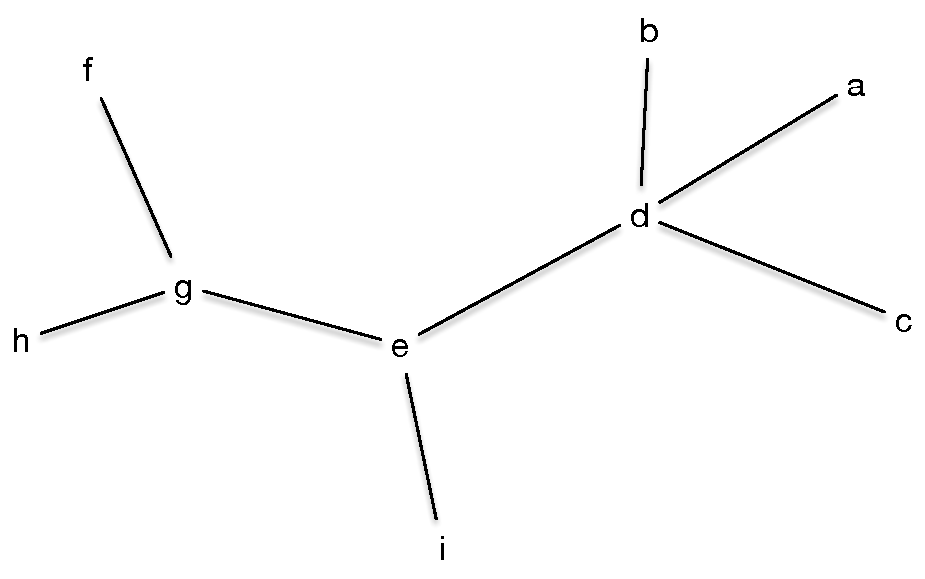
\includegraphics[scale=0.45]{arbre.pdf}
			\caption{Un arbre\label{arbre}} 
		\end{center}
	\end{figure}

	\begin{partie}

		\begin{questionpartie}
			Explicitez les feuilles et les sommets intérieurs de l'arbre de la figure~\ref{arbre}.
		\end{questionpartie}
		\begin{questionpartie}
			Donnez tous les splits de l'arbre de la figure~\ref{arbre}.
		\end{questionpartie}
	\end{partie}

	\begin{partie}
		\label{split-feuille}
		\begin{questionpartie}
			Donnez une condition nécessaire et suffisante pour qu'un split corresponde à la suppression de l'arête reliant une feuille au reste de l'arbre.
		\end{questionpartie}
		\begin{questionpartie}
			Montrez que si $x$ est une feuille de $T$ et que $xy$ est l'arête la reliant à $T$ alors le seul split séparant $x$ de $y$ ($x \in V_1$ et $y\in V_2$ pour un split $\{V_1, V_2\}$) est celui correspondant à la suppression de l'arête $xy$.
		\end{questionpartie}

		\begin{questionpartie}
			Vérifiez le pour la feuille $i$ de l'arbre de la figure~\ref{arbre}.
		\end{questionpartie}
		\begin{questionpartie}
			Soit $T'$ l'arbre resultant de la suppression d'une feuille de $T$. Comment déterminer les splits de $T'$ avec les splits de $T$ ?
		\end{questionpartie}
	\end{partie}	
	\begin{partie}
		\begin{questionpartie}
			Utilisez la partie~\ref{split-feuille} pour proposer une procédure permettant de reconstruire un arbre uniquement à partir de ses splits.
		\end{questionpartie}
		
		\begin{questionpartie}
			Quelle est la complexité de la procédure utilisée à la question précédente ?
		\end{questionpartie}
	\end{partie}	

\end{exo}

\begin{exo}[Condition nécessaire]
Soit $X$ un ensemble. On dit que $\mathcal{F} \subseteq \mathcal{P}(X)$ ($\mathcal{F}$ est un ensemble de sous-ensembles de $X$) est une {\bf\em famille complémentée sur $X$} si :
\begin{itemize}
	\item $\emptyset \notin \mathcal{F}$,
	\item $A \in \mathcal{F}$ implique que $\overline{A} = X \backslash A \in \mathcal{F}$.
\end{itemize}

\begin{question}
	Montrez que toute famille complémentée possède un nombre pair d'éléments et que l'union des splits d'un arbre  (si $\{V_1, V_2\}$ est un split de $T$, alors $V_1 \in \mathcal{F}$ {\bf et} $V_2 \in \mathcal{F}$) est une famille complémentée de $2(n-1)$ éléments.
\end{question}

\begin{question}
	\label{famille-buneman-1}
	Montrez que si une famille complémentée $\mathcal{F}$ sur $V$ est l'union des splits d'un arbre $T=(V, E)$, alors pour tous $A, B \in \mathcal{F}$ l'une des quatre assertion suivante est vérifiée :
\begin{itemize}
\item $A \cap B = \emptyset$
\item $A \cap \overline{B} = \emptyset$
\item $\overline{A} \cap B = \emptyset$
\item $\overline{A} \cap \overline{B} = \emptyset$
\end{itemize}	
	
\end{question}

\begin{question}
	Explicitez la question précédente sur l'exemple de la figure~\ref{arbre} en prenant des éléments de deux splits que vous choisirez.
\end{question}
\begin{question}
	\label{famille-buneman-2}
	Montrez que si une famille complémentée $\mathcal{F}$ sur $V$ est l'union des splits d'un arbre $T=(V, E)$, alors pour tout $x \in V$ : l'intersection de tous les $A \in \mathcal{F}$ contenant $x$ vaut $\{x\}$.
\end{question}

\end{exo}

\begin{exo}[Une condition suffisante]
	On appelle {\bf\em famille de Buneman} une famille complémentée satisfaisant les conditions des deux questions~\ref{famille-buneman-1} {\bf et}~\ref{famille-buneman-2}.
	\begin{partie}
		\label{hierarchie}
		On appelle {\em \bf hiérarchie} sur un ensemble $X$, un ensemble $\mathcal{H} \subseteq 2^X$ tel que $A, B \in \mathcal{H}$ implique $A \cap B \in \{\emptyset, A, B \}$ (les deux ensembles $A$ et $B$ sont soit disjoints soit inclus l'un dans l'autre).
		\begin{questionpartie}
			Montrez que si $\mathcal{H}$ est une hiérarchie, alors le graphe $G = (\mathcal{H}, E)$ tel que $\{A, B\} \in E$ si $A \subsetneq B$ et qu'il n'existe pas $C \in \mathcal{H}$ avec $A \subsetneq C \subsetneq B$ est un arbre.
		\end{questionpartie}
		\begin{questionpartie}
			Montrez que si $\mathcal{F}$ est une famille de Buneman sur $X$ alors l'ensemble $\mathcal{F}[A] = \{ B \vert B \in \mathcal{F}, B \subseteq A \}$ est une hiérarchie pour tout $A\in \mathcal{F}$.
		\end{questionpartie}
		\begin{questionpartie}
			Explicitez la question précédente en utilisant l'arbre de la figure~\ref{arbre} et en utilisant le split formé par la suppression de l'arête $\{d, e\}$ (montrez les deux hiérarchies).
		\end{questionpartie}

	\end{partie}
	\begin{partie}
		\label{unique}
		On suppose de plus ici que $\mathcal{F}$ est une famille de Buneman telle que pour tout $A\in \mathcal{F}$, il existe $x \in A$ tel que si $x \in B \in \mathcal{F}[A]$, alors $B = A$. On les appellera {\bf\em familles de Buneman strictes}.
		\begin{questionpartie}
			Montrer que l'union des splits d'un arbre $T=(V, E)$ est une famille de Buneman stricte.
		\end{questionpartie}
		\begin{questionpartie}
			Montrez que pour une famille de Buneman $\mathcal{F}$, s'il existe $x \in A$ tel que $x \in B \in \mathcal{F}[A]$ implique $B = A$, alors $x$ est unique.
		\end{questionpartie}
		\begin{questionpartie}
			Montrer que pour toute famille de Buneman stricte, il existe $x \in X$ tel que $\{x \} \in \mathcal{F}$.
		\end{questionpartie}
		\begin{questionpartie}
			\label{reconstruction}
		Utilisez les résultats de la partie~\ref{hierarchie} pour montrer que $\mathcal{F}$ est une famille de Buneman stricte sur $V$ si et seulement si il existe un arbre $T=(V, E)$ dont l'union des splits vaut $\mathcal{F}$.
		\end{questionpartie}	
	\begin{questionpartie}
		Explicitez la construction de la question précédente en utilisant l'arbre de la figure~\ref{arbre} (reconstruisez l'arbre à partir de ses splits).
	\end{questionpartie}

	\end{partie}

\end{exo}

\begin{exo}[Théorème de Buneman]

	On peut maintenant énoncer le théorème de Buneman qui ne présuppose pas que les familles soient strictes.
	\begin{question}
		Quel problème peut poser le fait qu'une famille de Buneman ne soit pas stricte pour la reconstruction de la question~\ref{reconstruction}  ? 
	\end{question}
	\begin{question}
		Proposez un moyen de transformer une famille de Buneman quelconque en une famille de Buneman stricte.
	\end{question}
	\begin{question}
		En déduire une procédure permettant d'associer un arbre à une famille une famille de Buneman.
	\end{question}

	\begin{question}
		Montrez que l'on peut reconstruire l'arbre de la figure~\ref{arbre} uniquement avec la famille $\{ A \cap F \vert A \in \mathcal{F}\}$ où :

		\begin{itemize}
			\item $F$ est l'ensemble des feuilles de l'arbre,
			\item $\mathcal{F}$ est la famille complémentée associée à l'arbre.
		\end{itemize}
	\end{question}
	\begin{question}
		As-t-on vraiment besoin de la condition de la question~\ref{famille-buneman-2} ou peut-t-on se contenter de la condition de la question~\ref{famille-buneman-1} ?
	\end{question}

\end{exo}

\end{document}
